\chapter{Balance bar}

\section{Introduction}
Generally cars have 60\% braking force front biased and 40\% rear biased, this is because the dynamic weight transfer is in front while braking.\\
In lay man's terms, front weight increases during brake, thus requiring more energy to stop. Hence balanced bar is used.\\
\section{Designing}
\section{First Iteration}
We designed our own balance bar because this allows us to make it according to the dimensions we need. It also reduces the cost as manufacturing a balance bar is relatively cheaper than buying one.\\
The balance bar was made according to the dimensions derived from the available bearing and female rod ends. Stress analysis was carried out on solidworks to see if it can bear the force on it during braking.
\begin{figure}[htb]
	\centering
	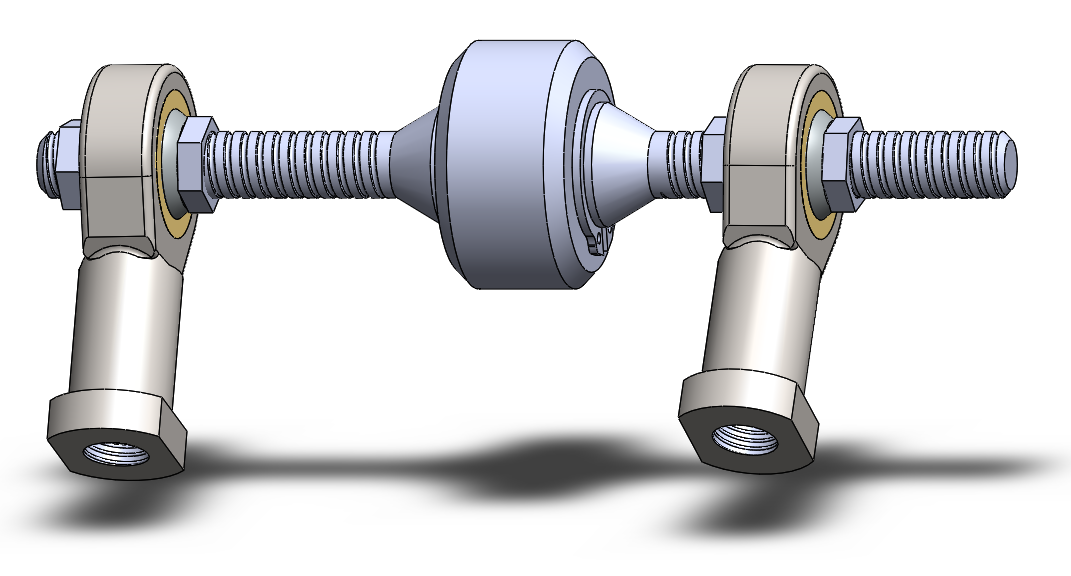
\includegraphics[scale=0.35]{fig/bb}
	\caption{Balance Bar}
	\label{fig:label}
\end{figure}

